\scanpage{258}
Considérons l'hom canonique
\[
\varphi:\operatorname{Pic}(X_y)\longrightarrow\operatorname{Pic}(\widehat X_y)
\]
(i) Le syst. projectif $(\operatorname{Pic}(X_n))_{n\in\mathbb Z}$ satisfait M.L.

\inserted{(ii) $\operatorname{Pic}(X_y)$ et $\operatorname{Pic}(\widehat X_y)$ ont $=$ image dans $\operatorname{Pic}(X_n)$, $\unsure{\forall n|\varphi}$.}

(iii) Pour que $\varphi$ soit \unsure{surjectif}, il f. et s. que $y$ soit un pt isolé du supp $R^1f_*(\mathcal O_X)$ \deleted{\unsure{en $y$}}.

(Cette condition est vérifiée en particulier si $X|(Y-\{y\})\longrightarrow Y-\{y\}$ est un isom.).

\margin{\unsure{Pour tout $n$}, de façon plus précise, $\exists k$ tel que \deleted{\unsure{les}} $H^1(X_{n+k},\mathcal O_{X_{n+k}}^*)$ et $R^1f_*(\mathcal O_X^*)_y$ aient $=$ image dans $H^1(X_n,\mathcal O_{X_n}^*)$}
\figure{\begin{tikzpicture}[x=1cm,y=1cm]\draw (0,0)--(0,4);\end{tikzpicture}}
\margin{\deleted{\unsure{Corollaire}}}

\deleted{\uline{Corollaire} 1.10 \deleted{Supposons que les} \deleted{\unsure{des espaces analytiques}} les $X_n$ soient ``algébrisables'', \deleted{et donc} se proviennent de schémas propres $\mathfrak X_n$ sur les $\mathfrak Y_n=\operatorname{Spec}\mathcal O_y/\mathfrak m_y^{n+1}$. Soit $\mathfrak X$ le schéma formel propre sur $\widehat{\mathcal O}_y$ défini par le système inductif des $\mathfrak X_n$. Supposons \deleted{de plus} \deleted{que $\mathfrak X$ sur $\widehat{\mathcal O}_y$ soit} que $y$ soit un pt isolé de $R^1f(\mathcal O_X)$.

\deleted{Deux} Conditions équivalentes :

(i) Il existe un voisinage ouvert $U$ de $y$ tel que $X|U$ soit projectif sur $U$ (\deleted{\unsure{Séminaire}} \unsure{Sém.} Cartan 1960/61).

(ii) \deleted{$\unsure{\mathfrak X}$ \illegible{2}}

b) \deleted{$\mathfrak X$ est algébrisable}}
\figure{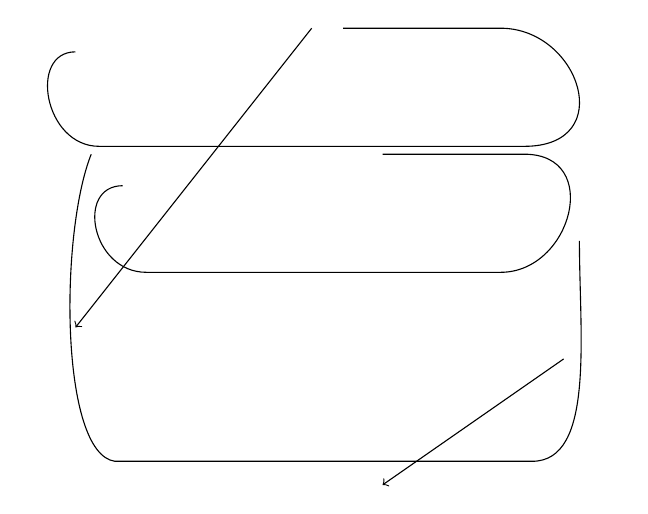
\begin{tikzpicture}[x=1cm,y=1cm]
\draw (0.1,5.5) .. controls (-0.5,5.5) and (-0.3,4.3) .. (0.4,4.3) -- (5.8,4.3) .. controls (7,4.3) and (6.5,5.8) .. (5.5,5.8) -- (3.5,5.8);
\draw (0.7,3.8) .. controls (0.1,3.8) and (0.3,2.7) .. (1,2.7) -- (5.5,2.7) .. controls (6.4,2.7) and (6.8,4.2) .. (5.8,4.2) -- (4,4.2);
\draw (0.3,4.2) .. controls (-0.1,3.2) and (-0.1,0.4) .. (0.6,0.3) -- (5.9,0.3) .. controls (6.7,0.3) and (6.5,1.9) .. (6.5,3.1);
\draw[->] (3.1,5.8) -- (0.1,2);
\draw[->] (6.3,1.6) -- (4,0);
\end{tikzpicture}}
\mspage{257}
